\chapter{Problems with Virtual Container Networks}
\label{chap:research}
%\emph{This chapter reports on the execution of the research method as described in an earlier chapter. If the research has been divided into phases, they are introduced, reported on and concluded individually. If needed, this chapter could be split up to balance out the sizes of all chapters.}
This chapter reports on the execution of the research to demonstrate what has been done. First we explain the current difficulties with managing virtual networks on \gls{dcos}. Next we explain the approach how another popular container orchestration platform, Kubernetes, handles virtual networks. Last we explain the different approaches we explored to improve the maintainability and management of virtual networks on \gls{dcos} for the \gls{poc}.

\section{Current state of virtual networks in DC/OS}
\label{sec:current-state}
\Gls{dcos} provides virtual networks by itself as overlay networks which can be used by the Docker and Mesos containerizer. This overlay is prepacked and enabled by default on the cluster. \Gls{cni} plugins are also supported on \gls{dcos} and can be used by both containerizers.

\subsection{DC/OS virtual networks}
\label{subsec:dcos-virtual-networks}
The overlay network was introduced to enable an IP-per-container model in \gls{dcos}. This allows operators to run applications on the default ports without worrying about port conflicts. This is done by creating an overlay network using \gls{vxlan}\cite{mahalingam2014virtual} which is supported by the Linux kernel. It works by creating two network bridges on each host, one for each containerizer. Containers on the same host and bridge can communicate directly with each other over the network bridge. A packet from a Mesos container to a Docker container on the same host will be routed through both bridges. A packet from a Mesos container on Agent~1 to a Docker container on Agent~2 follows a different path. First the packet will be routed to the Mesos bridge, the host's network stack consumes the package and encapsulates using \gls{vxlan} on Agent~1. Next Agent~2 decapsulates this packet and sends it up to the Docker bridge to be sent to the Docker container as can be seen in Figure~\ref{fig:dcos-overlay-arch}. 
\todo[inline]{Also add to this section that under the hood it is using CNI for UCR.}

\begin{figure}
    \centering
    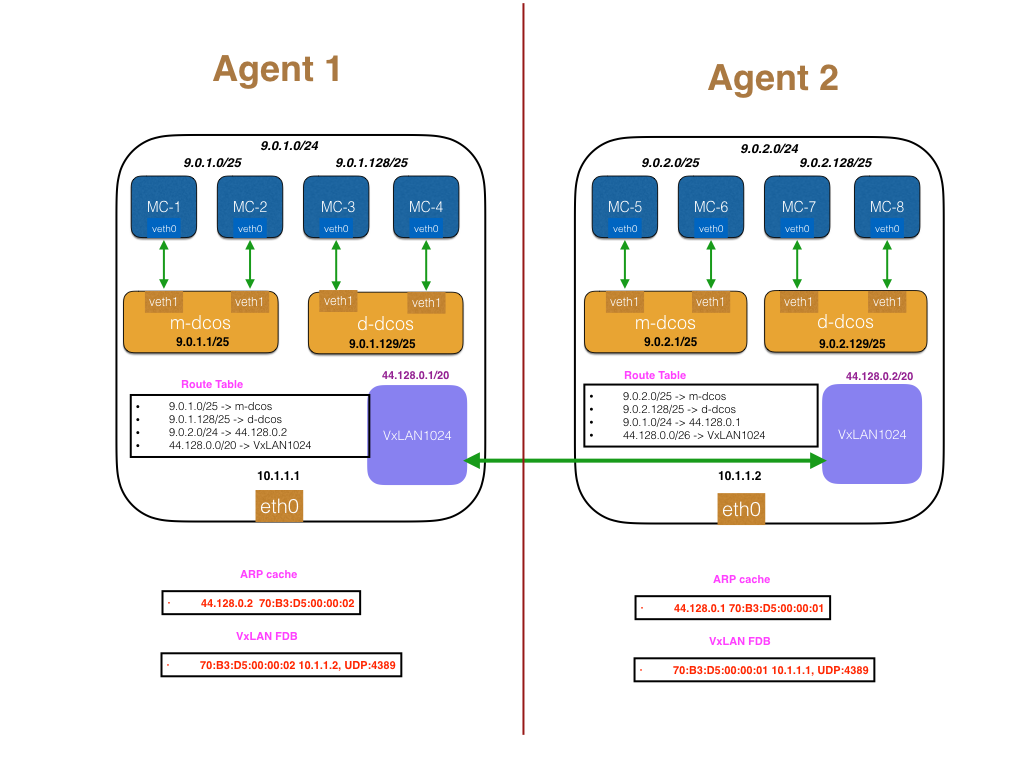
\includegraphics[width=1\columnwidth]{images/dcos-overlay-arch}
    \caption{DC/OS overlay in action\cite{dcos_overlay_arch}}
    \label{fig:dcos-overlay-arch}
\end{figure}

IP addresses are managed by the agent itself instead of a central location. A central location would require a reliably and consistent way of handing IP address assignment to containers in the cluster. The default configuration uses a \texttt{9.0.0.0/8} subnet, these are divided in smaller chunks, a \texttt{/24} to be managed by every agent itself. On the agent this subnet is divided into two equal subnets for each containerizer, resulting in 32 usable IP addresses for each container type on every agent. The agent's overlay module can request its allocated subnet from the overlay module running on the masters.

The default overlay network has the following limitations:
\begin{itemize}
    \item A limit on the number of usable IP addresses on each host, determined by the network prefix size. The default maximum is 32 Mesos and 32 Docker containers.
    \item Only IPv6 support for Docker containers, Mesos containers will fail to start.
    \item Operators are only able to create and delete virtual networks during installation of the cluster.
    \item The length of network names is limited as the Linux kernel only allows 15 characters for a network interface name.
    \item Marathon cannot execute healhtchecks in the default configurations as Marathon itself is not running on the virtual network.
    \item No \gls{api} to create and manage network policies on the virtual networks.
\end{itemize}

\subsection{CNI plugins on DC/OS}
\label{subsec:dcos-cni}
Too allow for more flexibility with virtual networks on \gls{dcos} operators can also chose to create virtual networks with other providers. Plugins following the \gls{cni} specification as discussed in Section~\ref{sec:cni} can be installed on \gls{dcos}. This works by placing the plugin in a dedicated folder on every agent. Networks can be created and configured by placing their relevant configuration files on every agent. Plugin location: \texttt{/opt/mesosphere/active/cni/} and configuration location: \texttt{/opt/mesosphere/etc/dcos/network/cni/}. A restart of the Mesos agent is required to make use of the new plugin or new configuration. \todo[inline]{find out if this still the case in newer versions.} The method mentioned above is only possible when using the Mesos containerizer. For Docker we need to create a Docker network on every agents with the \gls{cni} plugin as its driver.

Next any container can be launched on a virtual network by adding the following JSON to the configuration of the application: \texttt{\{"ipAddress": \{"networkName": "<<name>>"\}\}}. This will instruct the Mesos scheduler to request an IP address from that network using the configured \gls{cni} plugin. The plugin will take care of \gls{ipam} and creating and deleting of the network interface on the host machine. Depending on the features of the \gls{cni} plugin network policies can be applied by using the \gls{api} of the plugin.

The \gls{cni} plugin model for \gls{dcos} makes it flexible for operators to configure different virtual networks. However there is a drawback to this approach, as these networks are not visible to the operators and users of the cluster, as stated on the documentation\cite{dcos_sdn}:
\begin{displayquote}
    ``NOTE: The network tab currently displays information about containers that are associated with virtual networks managed by DC/OS overlay. It does not have information about containers running on virtual networks managed by any other CNI/CNM provider.'' 
\end{displayquote}
This makes it confusing for developers who want to deploy their applications. Colleagues on the client's project are having a hard time to understand how their applications are deployed and how to connect to them. Containers now live on a different network and are not always available on every machine. For example the SSH jumpbox used to connect to the cluster is not setup with Calico and is unaware of the virtual networks. As it does not have the routes in its route table to connect to the container workloads on a virtual network. 

There is also a problem with the different types of \gls{dns} providers within \gls{dcos}. The mesos-dns component provides a \gls{fqdn} to every service with the following structure: \texttt{<service-name>.<group-name>.<framework-name>.mesos}. This domain name however returns the IP address of the host of the container. In the case that the container is running on a virtual network it will return the wrong IP address. A connection is not possible because the port is only in use on the container network interface, resulting in a time-out for a user request. The other \gls{dns} provider is dcos-dns providing different addresses based on the network type of the container, see the overview below.
\begin{itemize}
    \item \texttt{<service-name>-<group-name>.<framework-name>.containerip.dcos.thisdcos.directory}: In container or bridge mode this will return the IP address of the container, in host mode it returns the agent IP address.
    \item \texttt{<service-name>-<group-name>.<framework-name>.agentip.dcos.thisdcos.directory}: Alwas the agent IP address.
    \item \texttt{<service-name>-<group-name>.<framework-name>.autoip.dcos.thisdcos.directory}: Resolves to the most suitable IP address, the agent IP address when in host or bridge mode and the container IP address in container mode.
\end{itemize}
\todo[inline]{Maybe convert to table together with mesos-dns entry}

To summarise we have the following drawbacks of using \gls{cni} plugins on \gls{dcos} to create virtual networks:
\begin{itemize}
    \item No method to retrieve or select the virtual networks created with \gls{cni} in the \gls{dcos} web and command line interface.
    \item No generic method of configuring network policies, as each plugin provider has its own dedicated \gls{api}.
    \item An operator has to manually distribute the plugin and configuration files to every slave using custom build solutions.
    \item Different \gls{dns} providers return different IP addresses for container workloads on a virtual network.
\end{itemize}

\section{Virtual networks in Kubernetes}
\label{sec:k8s-virtual-networks}
There are different ways of connecting containers in Kubernetes. The most basic one is in a pod where containers in the same pod can communicate via localhost. Pods get their own unique IP address, preventing operators to deal with port mappings and linking services together. 
\todo[inline]{expand on K8S}